\setcounter{chapter}{ 5 }
\chapter{GC Station, Part 1 }

\subChapterTitle{``The Water Rats''} 

\deets{Ion}{Aug. 24, 2012}



\textit{Comments in (parentheses) are commentary about what's going on in game, but they are mostly editorial, not from any character's POV.}

\textit{Comments in {[}square brackets{]} are out of game.  Comments with}\textit{\textbf{ {[}XXX{]}}}\textit{ are gaps or errors that need fixing.}







\jumpHeadline{ SAC-09 } 


\sceneHeadline{Bunker: Hayley and Oliver }

Hayley asks Oliver about how to be \hl{rude without getting punished for it}\footnote{\textbf{Suko T }Or at least that's what she was trying to ask, who knows what actually made it through the Hayley filter. :P \textsubscript{08/31/12 11:01pm}}. Oliver tells her to learn where people's lines are and know how far you can push someone.  Hayley asks him how she is supposed to know where people's lines are without outright asking them, since that hasn't worked so well for her in the past.


\sceneHeadline{Ops Room:  }\underline{ Officers and Patrol Group 1 }

The alarm goes off to summon the team to the ops room.  Already present are: Morgan, Rook, Trenton, Swan \& ``Mom''\textbf{ {[}XXX: }\textbf{\hl{I didn't get her name down}}\footnote{\textbf{Suko T }I don't think it was said. She was described as ``middle aged'' I think. \textsubscript{08/31/12 11:02pm}}\textbf{{]}}.\textbf{  }They are having a hushed conversation and Trenton is grumbling.



The team arrives.  The table is large and the agents are all sitting at one end of it.  Jockeying for sitting commences, Jaya sitting across from Morgan, with Hayley next to her and Jonah next to Hayley.  Rook sits next to Morgan.  Everyone's sitting together except for Oliver, who sits at the other end of the long table.  Morgan complains coldly to Jaya about spreading her team too thin.  Unusually, Oliver responds to this directly by making his way back to the team seats without comment and without Jaya getting a chance to say anything.  (One assumes his previous conversation with Morgan has something to do with it.)  \hl{Hayley gives up her seat for Oliver}\footnote{\textbf{Suko T }Protocol! \textsubscript{08/31/12 10:30pm}} and sits on the other side of Jonah.



Morgan claims that ``learning from past mistakes'' the agents will give the patrol information about their mission and ... let them decide for themselves if it is enough to go on.  They have the option to refuse.  \hl{(Whether that's actually an option is not so obvious: Morgan and Rook both make it clear later that time is absolutely of the essence, and attempts to take time to plan are clearly not looked upon favorably.)}\footnote{\textbf{Nathaniel Ford }I may have been unclear here; the intended effect was 'you can take your time, but the more time taken, the less value it has'. Morgan, naturally, wants the most value. ;-) \textsubscript{09/4/12 }}



The actual mission is ``GC Station''.  It had no service for many years up until the war, when both the Directorate and Nickelpan made inroads there.  The SAC-09 officers are interested because there is a facility with information they want: mostly personnel files, but also schematics, and actual tech.   It's an occupied (inhabited) area: savage people who have some source of sustenance that appears to be neither of the above polities.  The briefers are specifically interested in facility located in a notable landmark: a larger shaft going deep underground.



\textit{{[}At this point there was The Incident with the Jam.  It was to be one of several.{]}}



At this point Morgan asks for questions from the patrol.
{
\parskip=0pt
\begin{itemize}
\item Oliver: What is the purpose of the facility?
\end{itemize}

Morgan: Dissemination of information.  (What information and who it is disseminated to is not said.)

\begin{itemize}
\item Jaya: Are there adequate maps to go in and get back?
\end{itemize}

Morgan: No.

\begin{itemize}
\item Jaya: How do we carry things?
\end{itemize}

Trenton will be going on the mission in order to test devices found.  (Trenton is\textit{ thrilled} about this... or not.)

\begin{itemize}
\item Jonah: Is the mission several runs then?  Or is it a scouting mission?
\end{itemize}

Morgan: Up to you.  There won't be much to carry.

\begin{itemize}
\item Jonah: How long should the mission take then?
\end{itemize}

Morgan: Not more than a day.

\begin{itemize}
\item Oliver: Is the facility in the shaft occupied by the locals?
\end{itemize}

Morgan: Not as far as we know.

\begin{itemize}
\item Oliver: How old is this information?
\end{itemize}

Morgan: Several years.  (Good to know!)  The source is Nicklepan.

\begin{itemize}
\item Oliver: What about Anglia?  Are they involved?
\end{itemize}

Morgan: There is a strong likelihood Anglia knows about it.  However we don't think they are interested.

\begin{itemize}
\item Jonah: How do we recognize what we need?
\end{itemize}

Morgan shows the patrol \hl{a hand-drawn picture of stoppered vials with blotches on them, in a rack}\footnote{\textbf{Nathaniel Ford }To clarify, the picture was of stoppered vials, and a rack of slides with blotches on them. \textsubscript{09/04/12 4:25pm}}.  The picture is provided by Trenton.

\begin{itemize}
\item There is some back and forth between Jaya, Oliver and Jonah about how to carry the vials.  This appears to annoy Trenton.
\item Jonah:  How much time is there to prepare for the mission?
\end{itemize}

Rook: None really.  (It appears overall that leopards don't change their spots very much.)
}


Jaya accepts the mission without hesitation.  Unsurprisingly none of the others say otherwise.  \hl{Jonah tries to ask Rook about further preparation or advice after Morgan leaves.}\footnote{\textbf{Adam Kenney }Does anyone remember the exact question that blew Rook's mind?  I seem to recall that it was a strangely specific topic, I think about trains, but I can't remember exactly. \textsubscript{09/02/12 7:42am}}\footnote{$\rightarrow$\textbf{q.google }Actually now that you mention it... the question was initially about whether we would have preparation time at base.  When the answer was (I think) negative it changed to whether we would have preparation time on the train.  But it was phrased as asking *how long the trip would be*. \textsubscript{09/02/12 12:39pm}}\footnote{$\rightarrow$\textbf{Adam Kenney }Yes, that's right!  What you asked him was how long the trip would be.  He 
asked like you asked the distance between the two moons or something. 

    Adam  \textsubscript{09/02/12}}
 
This seems to stymie Rook, though whether it's from uncertainty, indignation at being asked, or some other cause Jonah is not able to tell.   Jonah behaves as if asking is perfectly normal and that he is satisfied with Rook's lack of an answer.


\sceneHeadline{The Requisition Cage }

The team equips:

\begin{itemize}
\item Jaya:\textit{ Transit Authority Patrol Uniform} (1),  \textit{Medkit} (1)
\item Oliver:\textit{ Radio Network} (2),\textit{ Urban Camouflage} (1),\textit{ Medkit} (1)
\item Jonah:\textit{ Transit Authority Patrol Uniform} (1),\textit{  Rifle} (1)
\item Hayley:\textit{ Transit Authority Battle Dress Uniform} (2)
\end{itemize}



There is some friendly banter with Jari.  Oliver asks Jari if he fought in the war, to which Jari replies he's fought in\textit{ a} war.  This is not the first time the team has heard this from residents of SAC-09 (Morgan) but Jari politely but firmly drops the subject.  \textbf{{[}XXX: If anything else was important, fill it in.  I don't remember it.{]}}  There is also some furniture at the station as the team leaves.  Oliver asks Rook about the furniture coming on the train, but \hl{Rook says it's not being brought on the train it's being brought\textit{ off}.}\footnote{\textbf{Adam Kenney }Oliver digs a bit about ``reinforcements?'' and Rook says something along the lines of, ``that's a good thing''. \textsubscript{09/02/12 7:44am}}  Rook does not elaborate further.



\sceneHeadline{Train } 



Trenton boards late, all of us have been waiting around for some time before he shows up.  He quickly sets up shop on the train in Grand Style: a large comfortable chair to sit on, and numerous cans (of what is likely beer – but only Oliver and possibly Hayley would recognize it as such.  The idea of canning is beyond Jonah and Jaya's experience. )  Trenton makes it clear that he intends to stay there for the remainder of the trip.  Jaya and Trenton spar \textbf{{[}XXX: Over what is unclear.  }\textbf{\hl{It appears to be lack of discipline.}}\footnote{\textbf{Nathaniel Ford }So, who actually has less discipline? What do the viewers at home think? \textsubscript{11/07/14 7:25pm}}\textbf{{]}} and Jaya spends most of the trip deliberately ignoring Trenton.  \hl{Hayley had helped set up Trenton's chair and doesn't speak much, mostly just watching Trenton with an odd expression.  She doesn't seem to notice Jaya glaring at her.}\footnote{\textbf{Nathaniel Ford }In light of Drake this behavior pattern is pleasingly repeated. \textsubscript{11/07/14 7:27pm}}\footnote{$\rightarrow$\textbf{Suko T }Hayley is always very consistent!  Until she isn't. \textsubscript{11/08/14 10:53pm}}  Jonah asks Trenton about what they are looking for and learns that Trenton doesn't know either – or at least sees some value in refusing to actually say.  Jonah emphasizes that none of the patrol are in a position to really guess, and they have limited carrying capacity.  Trenton answers that he can always be asked about it by radio.  (That's optimism for you.)



The train once again does that disorienting, nauseating lurch when it seems to have reached top speed.



\sceneHeadline{ GC Station } 



As the team leaves the train, Hayley lingers behind and seems to come to some sort of decision.  \hl{She takes a deep breath, looks Trenton in the eye and says: ``Don't die,`` and then squeezes her eyes shut for some reason.}\footnote{\textbf{Nathaniel Ford }WHAT WAS THE REASON!? \textsubscript{11/07/14 7:28pm}}\footnote{$\rightarrow$\textbf{Suko T }She was ordered not to talk to Trenton, or even look at him, so she is breaking both orders and is utterly terrified and somewhat nauseated at her daring.  But for Signe, for her only friend (at that point), she would do anything.  She's also trying to limit the amount of time that she is actually breaking the orders (hence eyes shut and two word sentence)... the sooner to get the emotional dissonance over with. \textsubscript{11/08/14 10:52pm}}\footnote{$\rightarrow$\textbf{Nathaniel Ford }Ah, right! I'd forgotten she'd been ordered not to talk to him. \textsubscript{11/09/14 1:09pm}}\footnote{$\rightarrow$\textbf{Suko T }It certainly made things a little difficult/silly, particularly in session 10 when he tried to talk to her and she had to talk to a wall.  Hayley did confess to Jaya later (session 11) for all these violations so she could be properly punished.  Jaya declined. \textsubscript{11/09/14 2:59pm}}\footnote{$\rightarrow$\textbf{Nathaniel Ford }+1 \textsubscript{11/09/14 7:19pm}}  Trenton: ``I'd say the same to you – but I have a good feeling about this.''



Water drips from the tunnel walls.  What water we can see is black and noxious looking.    The air is damp.This makes the team nervous.  They head out.  Jonah discusses protocol with strangers with Jaya.  Hayley asks Jaya about keeping Oliver from being noticed as one of the TA (due to the urban camo ironically) by sending him off separately.  Jaya says that when its appropriate she'll send Oliver off.  Oliver says that he likes Jaya's company which surprises Hayley.  Oliver winks at Hayley.  Jonah explains Oliver and Jaya like to dislike each other.



Climbing up the rubble to an opening. Jaya and Hayley climb ahead and give the all clear.  Not sure of the direction at the top but the team heads ``north''.  The marching order: Jonah, Jaya, Hayley, Oliver.  The passage narrows then widens out to daylight coming down from above. The lit area is circular with ruins all around and open sky.  There are no obvious exits.  Jonah has a bad feeling and the patrol backs up into the tunnel.  As they are backing up they hear a grinding noise down the tunnel, like the huge metal door to SAC-09 closing up ahead as they retreat.  Oliver tries to inform Trenton by radio, but Trenton doesn't care. Jaya sends Hayley and Oliver back to the open area to investigate it for exits.  Jaya and Jonah find that hallway is sealed by a piece of metal that fits remarkably well for blocking it.  Someone has closed the patrol in.



\textit{{[}The Water Rats enter the threat pool{]}}



Scanning the circular area Oliver notices a kid watching them from the perimeter\textit{ {[}Challenge: Notice the watcher up above{]}}.  Oliver \& Jonah spot a kid laying down canvas from a gap in the wall.  Oliver hails him: ``We're here from the Transit Authority!''\textit{ {[}Opening: Reveal team to water rats{]}.}  Someone scrambles up above the upper edge to look at the patrol and then drops behind again.  Hayley warns Jaya the position is not defensible.  Jaya asks her to find out if she can climb it.



A voice calls: ``Where you from?''.  Oliver replies ``From the Directorate.  We're just passing through.''  The voice seems rather inclined to disbelieve him.  He asks about the group's intentions, and Oliver tells him they are looking for a lost thing, and asks the way to the surface.  They banter.  It's clear the locals don't trust the patrol, don't want them there, believe they might be from Nicklepan (who they appear to be hostile to), and certainly aren't going to let them go forward\textit{ or} back, citing the ``bad position'' the patrol is in.  They want payment for the patrol to be allowed to go anywhere safely.



Oliver acts nonchalant at this, behaving like the team is used to this sort of thing and isn't really concerned or afraid of the speakers\textit{ {[}Challenge: Veteran bluff{]}}.  The team then pushes back at the speakers, joking about supposed previous encounters, laughing at the thought that they might be in any danger and generally trying to intimidate the locals\textit{ {[}Challenge: Intimidate the Water Rats{]}}.  They bargain with Jaya noting that while the aren't interested in the threats they\textit{ would} be interested in hiring a guide.  This mostly works despite occasional ``translation problems''\textit{ {[}Opening: Misheard words{]}}.  Meanwhile Hayley scans the walls for ways to climb up and tells Oliver where they are so he can cover her if she has to make a sudden break for the walls to climb to one of the openings they can see.  Any way out would involve a lot of athleticism.  There is clearly some jumping involved, which Oliver probably can't do with his leg, but even for the others its an exposed position.



A gravelly voiced man (Raj) with a couple of flankers comes down ropes to negotiate.  The team initially agrees to give the locals smokes, money, a flashlight, medical supplies and a rifle, in return for being allowed up and getting a local guide to the enormous shaft in the ground\textit{ {[}Challenge: Trading with the Water Rats{]}}. Jonah calls their attention to antibiotics\textit{ {[}Challenge: Notice the medical needs of the water rats{]}}. He also talks them out of the rifle: ``We're soldiers like you.  We fought Nicklepan like you.   You can have our smokes, medical supplies and money but we're not going anywhere unarmed.''  The negotiators seem satisfied enough with the other goods (they try out the smokes... and the money), and they accept the bargain.  There is some discussion of Nicklepan, whom the locals seem unfriendly toward, and some fishing about the nature of the Directorate, which Oliver handles by being blunt\textit{ {[}Opening: Contradicting the trader{]}.}



The patrol climbs the ropes up out of the shaft.  Hayley climbs up first.  On the other side is an encampment or village with 30-40 people of various ages – but all male, and all\textit{ quite} interested in Hayley.  They are less excited by Oliver, who climbs up next, and even less so by Jonah, who follows.  Jaya elicits startled looks and backing away hurriedly\textit{ {[}Opening: Scaring the kids{]}}.  (They \textit{are} picky apparently).



The patrol meets the locals.  Hayley is introduced to the rather friendly Nigel.  They proceed to talk past each other, Hayley asking if he is Franchise, which he doesn't seem to understand, eventually saying ``we're free men''.  (They certainly can't charge anything.)  Oliver is aloof: The buildings in the area are not quite level (the water has risen below them) and many of them are bombed out shells, which takes Oliver back to a bad place\textit{ {[}Opening: Distracted by bombed out buildings{]}}.  After getting over their initial shock the locals decide that they do in fact find Jaya disturbing, mistaking her look of official seriousness for scowling\textit{ {[}Opening: Off-putting attitude to Water Rats{]}}.  Jonah gets to know people, playing up the war experiences of the group and referencing Oliver and Jaya particularly as veterans.



Hayley notices a bald, scowling man watching them in distinctly less-friendly fashion than the others \textit{{[}Challenge: Notice Vic{]}.  }She drifts closer to get a better look.  More people flirt with her.   Somebody grabs at her ass, and she reacts by throwing them\textit{ {[}Challenge: Notice threatening little hands{]}}.  It turns out to be a small child who flies some distance.  A big guy (the kid's father it turns out) reacts badly and interrogates Hayley roughly.  This doesn't work as he expects, but Hayley downplays the situation.  The big guy eventually retreats to the vicinity of the scowling bald man.



The team meets their guide, Jayce, who leads them away from the crowd.  Jayce is mostly friendly enough, though he warns the team not to draw weapons, to get rid of any explosives and not to make any loud noises (the latter two are connected as becomes apparent later).  He says if we ``fuck up, we'll send you to the Lady. She runs things around here.''



He expresses mild disbelief that they ``really want to go towards that hole''.  Jaya flirts with him, which is apparently enough to overcome her previous first impression.   Jayce makes it clear that he'll lead the patrol to the shaft but he's not going down it.  The team reassures him that that will be sufficient, with Jonah trying to offer some incentive for him to wait a while for their return.



Jayce asks Hayley about what the kid did and why it surprises her.  She replies she simply wasn't expecting it, to which Jayce, both not-quite-believing her and teasingly asks what she does when she\textit{ does} expect it.  This becomes a little more than anyone was planning for, as Hayley starts negotiating to find out what he would pay.  Jaya reacts badly to this and after some angry words she eventually orders Hayley to stop.  (Hayley later tells Jonah it was very unlikely Jayce could afford her, but that it was worth finding out as a bargaining point.  Jonah appreciates this attitude more than Jaya does.)  Oliver changes the subject, asking Jayce about aforementioned scowling bald guy, named Vic.  Vic apparently works for the Lady.  Oliver asks what the Lady has, to which Jayce explains that she is The Woman.  Not\textit{ a} woman,\textit{ The} Woman, the one and only woman in the camp.  There are no others.  Oliver asks where the kids come from then.  Jayce gives him a look and very carefully says ``the Lady''.  He implies that women around here disappear.  Girl children too.  (It's not explained but the impression is given that the Lady is\textit{ not friendly} to any competition, which explains why Hayley was being scowled at.  It's not until slightly later that any explanations other than hard-core rivalry are brought up.)



Oliver moves to asking more about Nicklepan, the war and the area in general.  Jayce explains that the buildings in the area have become\textit{ rather unstable}, prone to falling down catastrophically when there are\textit{ any} loud noises.  (Which is why he warned about not having explosives or making loud noises).  He seems to attribute this to the war with Nicklepan, though whether it is caused\textit{ by} Nicklepan or is the local reaction\textit{ to} Nicklepan is unclear.  Certainly they have not come back in any numbers since the war.  Oliver asks about food.  Apparently the diet is mostly moss (poor pickings even by Franchise standards).  There are no klipspringers, as they've all died, no chickens either, but plenty of rabbits (which no one from the patrol has heard of).  Interestingly there are no chickens again because all the females die.  (Whether anyone makes the connection given how briefly it comes up is an open question.)  Why ``rabbits'' are immune is unclear, except that they ... breed with great vigor and frequency.   Oliver or Jonah brings up trade, to which Jayce smiles and says that they generally don't want anything from outsides – with the notable and obvious exception they've been talking about.  This captures Jonah's attention: clearly there is an opportunity here for bargaining, if not for profit then at least for getting out safely.



They walk for some distance and stop to eat and rest near a large Arch.  Jonah repacks the medkits to rebalance after the trade\textit{ {[}Opening: Redistribute medkits{]}.}  Hayley and Jonah talk about what was going on with Vic and the Lady since she didn't quite follow what was going on in that discussion.   Jaya shares her booze with Jayce, clearly in an unusually friendly mood.



While she stood there chatting with Jonah, Oliver notices someone jumping out at Hayley\textit{ {[}Challenge: Notice assault on Hayley{]}}.  He turns swiftly and shoots the assailant with his rifle, blowing his head open\textit{ {[}Challenge: Assault on Hayley{]}}.  Hayley actually ducks and covers (we were all so proud!) – with the corpse of the assailant\textit{ {[}Opening: Protect self instead of others{]}.}  Jayce, taken totally by surprise, tries to draw a gun – which leads Jaya to think he's part of the attack.  She elbows him in the gut and jumps on him\textit{ {[}Challenge: Knocking Jayce down{]}}.  He draws a knife to her throat, while she wrestles him down\textit{ {[}Challenge: Maintain dominant position in grapple{]}}.  (This all could've been\textit{ so much better} if the circumstances were more private, and had more candlelight – or just more booze.)  She accuses him of setting them up, which he denies angrily.



Hayley hides.  Oliver shoulders his rifle and runs over to Hayley to make sure she's okay\textit{ {[}Opening: Shouldering gun{]}.}  Jonah tries to break up the fight, while Jaya pours oil it.  It takes some time to convince her that the only gunshot was Oliver defending Hayley.  Eventually things calm down and Jayce looks at the body, which does (did) in fact belong to one of Vic's men.  Jonah notices Jayce taking stuff off the body but as \hl{none of it is very important}\footnote{\textbf{Adam Kenney }We don't really know that, do we? \textsubscript{09/02/12 7:53am}}\footnote{$\rightarrow$\textbf{q.google }No we don't.  But it was just a 1-point challenge and it seemed to me that Nate treated the focus of it as noticing the theft rather than what in particular was stolen.  Nate, am I off base? \textsubscript{09/02/12 12:44pm}}\footnote{$\rightarrow$\textbf{Nathaniel Ford }Remember that challenges have to have narrative impact. If it was narratively important for him to steal it, but unimportant for you to stop him, or otherwise react, I would have said ``You notice him palm a few things.'' That's really him stealing stuff as flavor. Instead, the challenge  says, ``He is taking something. Noticing that he is gives you the opportunity to react; in turn, the reaction can change the overall narrative in a significant manner.'' \textsubscript{09/04/12 3:26pm}} he ignores it\textit{ {[}Challenge: Notice Jayce palming stuff from assaulter's corpse{]}}.  Unfortunately Jaya is still angry and shifts from blaming Jayce for setting them up to blaming him for not guiding them safely.   She yells at Jayce who says insulting things about her not being a mother which leads her to slug him\textit{ {[}Opening: Hitting Jayce for insult{]}}.   \hl{Oliver calms Jaya down}\footnote{\textbf{Adam Kenney }Not sure if anyone caught this - he almost acted like her commanding officer rather than the other way around during this exchange.  A little bit of Citizen showing through. \textsubscript{09/02/12 7:54am}}\footnote{$\rightarrow$\textbf{q.google }I didn't catch it.  It's good to mention these things.  I know I keep mentioning the rare breaks in Jonah's facade because they are rare, and I'm not a good enough actor to really convey the tension on his face or how quickly it comes and goes. \textsubscript{09/02/12 12:46pm}}\footnote{$\rightarrow$\textbf{Rebecca S. }I feel like somewhere in the future Oliver is going to get the flaw : ``Promoted'' \textsubscript{09/04/12 2:07pm}}\footnote{$\rightarrow$\textbf{Nathaniel Ford }Bwahaha! \textsubscript{09/04/12 3:27pm}}\footnote{$\rightarrow$\textbf{Suko T }Hee!  That would be a beautiful thing. \textsubscript{09/05/12 12:06am}}, while Jonah talks Jayce down.  Jonah is able to convince Jayce that backing out of the deal is not acceptable, but Jayce still is so angry at the way he's been treated that he abandons the group to their fate immediately after getting them to the shaft entrance where there is a rubble slope and three tunnels branching off at the bottom.



\hl{(Ah well.  It would never have worked anyway.  ``Jaya and Jayce'' would've been too confusing.)}\footnote{\textbf{Nathaniel Ford }Jury is still out... \textsubscript{11/07/14 7:45pm}}



\jumpHeadline{Challenges \&  Refreshes }  


{
\parskip=0pt
\begin{itemize}
\item Notice the watcher up above: 1.  \textit{Focused} (Oliver): 1,\textit{ Conceal} (Jonah): 1.   \textbf{Overcome: 1 VP} (Oliver).
\item \underline{ Refresh }: Reveal team to Water Rats:\textit{ Outgoing} (Oliver)
\item Veteran bluff: 2.  \textit{Outgoing} (Oliver): 2,\textit{ Veteran} (Oliver): 2.  \textbf{Overcome: 2 VP} (Oliver).
\item Intimidate the Water Rats: 3.\textit{  Grim Visage} (Jaya): 2,\textit{ Air of Command} (Jaya): 1,\textit{ Social Chameleon} (Jonah): 3,\textit{ Protocol} (Hayley): 1.  \textbf{Overcome: 1 VP} (Hayley),\textbf{ 1 VP} (Jaya),\textbf{ 1 VP} (Jonah).
\item \underline{ Refresh }: Mis-heard words: ``trader'' as ``traitor'':\textit{ Social Chameleon} (Jonah)
\item Trading with the Water Rats: 4.\textit{  Medkit} (Jaya): 1,\textit{ Family Money} (Oliver): 1,  \textit{Smokes} (Jaya): 1,\textit{ Uniform} (Jaya): 1,\textit{ Social Chameleon} (Jonah): 3.  Matched.
\item Notice the medical needs of the Water Rats: 1.  \textit{Street Medic} (Jonah): 2.  \textbf{Overcome: 1 VP} (Jonah).
\item \underline{ Refresh }: Contradicting the trader (``We don't have a Sultan''):\textit{ Outgoing} (Oliver).
\item Notice Vic: 1.  \textit{Ladies' Maid} (Hayley): 2.  \textbf{Overcome: 1 VP} (Hayley).
\item \underline{ Refresh }: Scaring the kids:\textit{ Grim Visage} (Jaya)
\item \underline{ Refresh }: Distracted by bombed out buildings:\textit{ Focused} (Oliver)
\item \underline{ Refresh }: Off-putting attitude to Water Rats:\textit{ Air of Command} (Jaya)
\item Notice threatening little hands: 1.  \textit{Bodyguard} (Hayley): 1.  Matched.
\item \underline{ Refresh }: Redistribute medkits:\textit{ Street Medic} (Jonah)
\item Notice assault on Hayley: 1.  \textit{Focused} (Oliver): 1.  Matched.
\item Assault on Hayley: 2.\textit{  Crack Shot} (Oliver): 3.  \textbf{Overcome: 2 VP} (Oliver).
\item \underline{ Refresh }: Protecting self rather than others:\textit{ Bodyguard} (Hayley).
\item Knocking Jayce down: 1.  \textit{Truncheon} (Jaya): 2.  \textbf{Overcome: 1 VP} (Jaya).
\item Maintain dominant position in grapple: 1.  \textit{Adrenaline Junkie} (Jaya): 2.  \textbf{Overcome: 1 VP} (Jaya).
\item \underline{ Refresh }: Shouldering gun before going to check on Hayley:\textit{ Crack Shot} (Oliver)
\item Notice Jayce palming stuff from assaulter's corpse: 1.  \textit{Vigilant} (Jonah):  \textbf{Overcome: 1 VP} (Jonah).
\item Hitting Jayce for insult about her womanhood:\textit{ Adrenaline Junkie} (Jaya)
\end{itemize}

}

\jumpHeadline{ Quotes }  


\quotedDialog{
Raj: So, yeah, the Directorate, aren't you the ones with the Sultan who likes tea?

Oliver: Not us.   We don't have a ...  Sultan?

Jonah: We have a Senate.

Raj (friendly sarcasm): Oh\textit{ yeah}.  That must be it.  A\textit{ Senate}.
}


``Don't worry.  Not all women hit that hard''.

\extraIndent{- Jonah, explaining the facts of life to Jayce}


\quotedDialog{
``Why would I stay with you?  You're two crazy bitches and a guy who can't get over the war.''

``And doesn't miss.''

``Good point.''
}
\extraIndent{ - Jayce and Jonah}



\textit{{[}}\textit{There was some other funny discussion between Jonah and Jayce about the nature of women (funnier given the ignorance of the Water Rats about same) but it wasn't written down.{]}}


\vspace{\fill}

\begin{flushright}
\textsubscript{last edited by \textbf{Nathaniel Ford} @ 05/07/15 4:28pm}
% Exported @ 08/22/15 1:30pm
\end{flushright}

\begin{center}
~
\vskip 0em
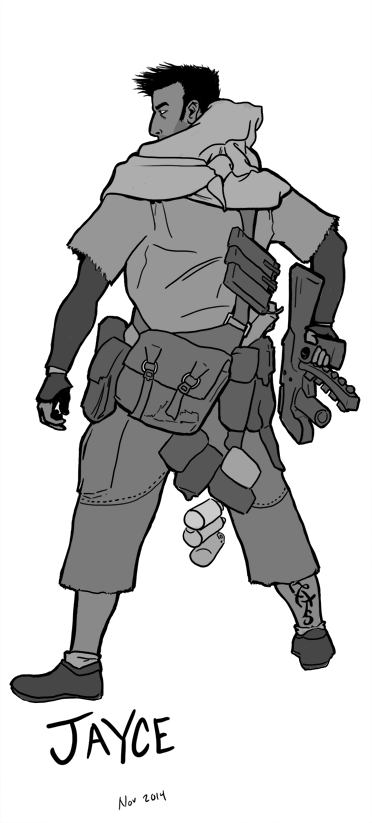
\includegraphics[width=8cm]{img/jayce.png}
\end{center}
